% Video-presentation slides, Part 2 (Mahbubur).
% Skeleton with topic placeholders. Fill in numbers/figures during rehearsal.
% Covers: results -> polari diagnostic -> uncertainty -> conclusion.
% Total target time: 5 minutes.

\documentclass[aspectratio=169,11pt]{beamer}

\usetheme{metropolis}
\usepackage{graphicx}
\usepackage{booktabs}
\usepackage{xcolor}

\definecolor{accent}{HTML}{1E64C8}
\definecolor{warn}{HTML}{C81E1E}
\setbeamercolor{progress bar}{fg=accent}
\setbeamercolor{frametitle}{bg=accent}

\title{Parameter-Efficient Adaptation of SAM~2 for\\Sentinel-1 SAR Flood Inundation Mapping\\in the Indo-Gangetic Region}
\subtitle{Part 2: Results and Diagnosis}
\author{Mahbubur Rahman \\ {\small Co-author: Aksan Gony Alif}}
\institute{BRAC University}
\date{}

\begin{document}

\maketitle

% ---------------------------------------------------------- Slide 1: Headline numbers
\begin{frame}{Headline results}
\begin{center}
\small
\begin{tabular}{lcccc}
\toprule
Method & Sen1F11 test & Bolivia & Pak-S1F11 & Pak-2022 \\
\midrule
U-Net baseline                & 0.601 & \textbf{0.684} & 0.271 & \textbf{0.672} \\
Hiera-B+ + AdaptFormer        & \textbf{0.634} & 0.458 & 0.254 & \textcolor{warn}{0.090} \\
Hiera-B+ + LoRA               & 0.599 & 0.635 & 0.255 & \textcolor{warn}{0.140} \\
Hiera-B+ + DoRA               & 0.602 & 0.637 & 0.254 & \textcolor{warn}{0.132} \\
\bottomrule
\end{tabular}
\end{center}
\vspace{0.6em}
\begin{itemize}
    \item \textbf{In-distribution:} AdaptFormer wins ($0.634$), beating U-Net at a fraction of trainable parameters.
    \item \textbf{Bolivia held-out:} DoRA matches U-Net ($0.637$ vs $0.684$).
    \item \textbf{Pakistan-2022:} every SAM-family cell collapses to \textcolor{warn}{$0.09$--$0.14$}, while U-Net retains $0.672$.
\end{itemize}
\end{frame}

% ---------------------------------------------------------- Slide 2: Setup the puzzle
\begin{frame}{The Pakistan-2022 collapse: not a backbone or adapter problem}
\begin{itemize}
    \item Every SAM-family cell collapses, regardless of:
    \begin{itemize}
        \item Backbone (ViT-Base, ViT-Large, ViT-Huge, Hiera-Base-Plus, Hiera-Large --- all collapse)
        \item PEFT method (LoRA, DoRA, Conv-LoRA, AdaptFormer --- all collapse)
        \item Random seed
    \end{itemize}
    \item U-Net on the same training data does not collapse. So the collapse is \emph{specific to the adapted SAM-family models}, not a property of the dataset.
    \item \textbf{Question:} what is the SAM family seeing that the U-Net is not?
\end{itemize}
\end{frame}

% ---------------------------------------------------------- Slide 3: The diagnostic
\begin{frame}{The polarimetric ablation: cross-polarization is the culprit}
\begin{center}
\small
\begin{tabular}{lcc}
\toprule
Pakistan-2022 IoU & Dual-polarization & Single-polarization (VV only) \\
\midrule
Hiera-B+ Conv-LoRA & $0.113$ & $\mathbf{0.632 \pm 0.057}$ \\
Hiera-B+ LoRA      & $0.144$ & $\mathbf{0.631 \pm 0.050}$ \\
Hiera-B+ DoRA      & $0.131$ & $\mathbf{0.658 \pm 0.014}$ \\
Hiera-B+ AdaptFormer & $0.092$ & $\mathbf{0.556 \pm 0.050}$ \\
\midrule
\emph{U-Net reference} & \multicolumn{2}{c}{$0.672$} \\
\bottomrule
\end{tabular}
\end{center}
\vspace{0.6em}
\textbf{Drop the cross-polarization (VH) channel and the collapse vanishes.}
\begin{itemize}
    \item Single-polarization Pakistan-2022 IoU jumps to $0.56$--$0.66$ across three seeds.
    \item Within $0.01$--$0.12$ of the U-Net baseline.
    \item \textbf{Three-seed evidence; no overlap with the dual-pol band.}
\end{itemize}
\end{frame}

% ---------------------------------------------------------- Slide 4: Qualitative figure
\begin{frame}{Qualitative comparison: same chip, three predictions}
\begin{center}
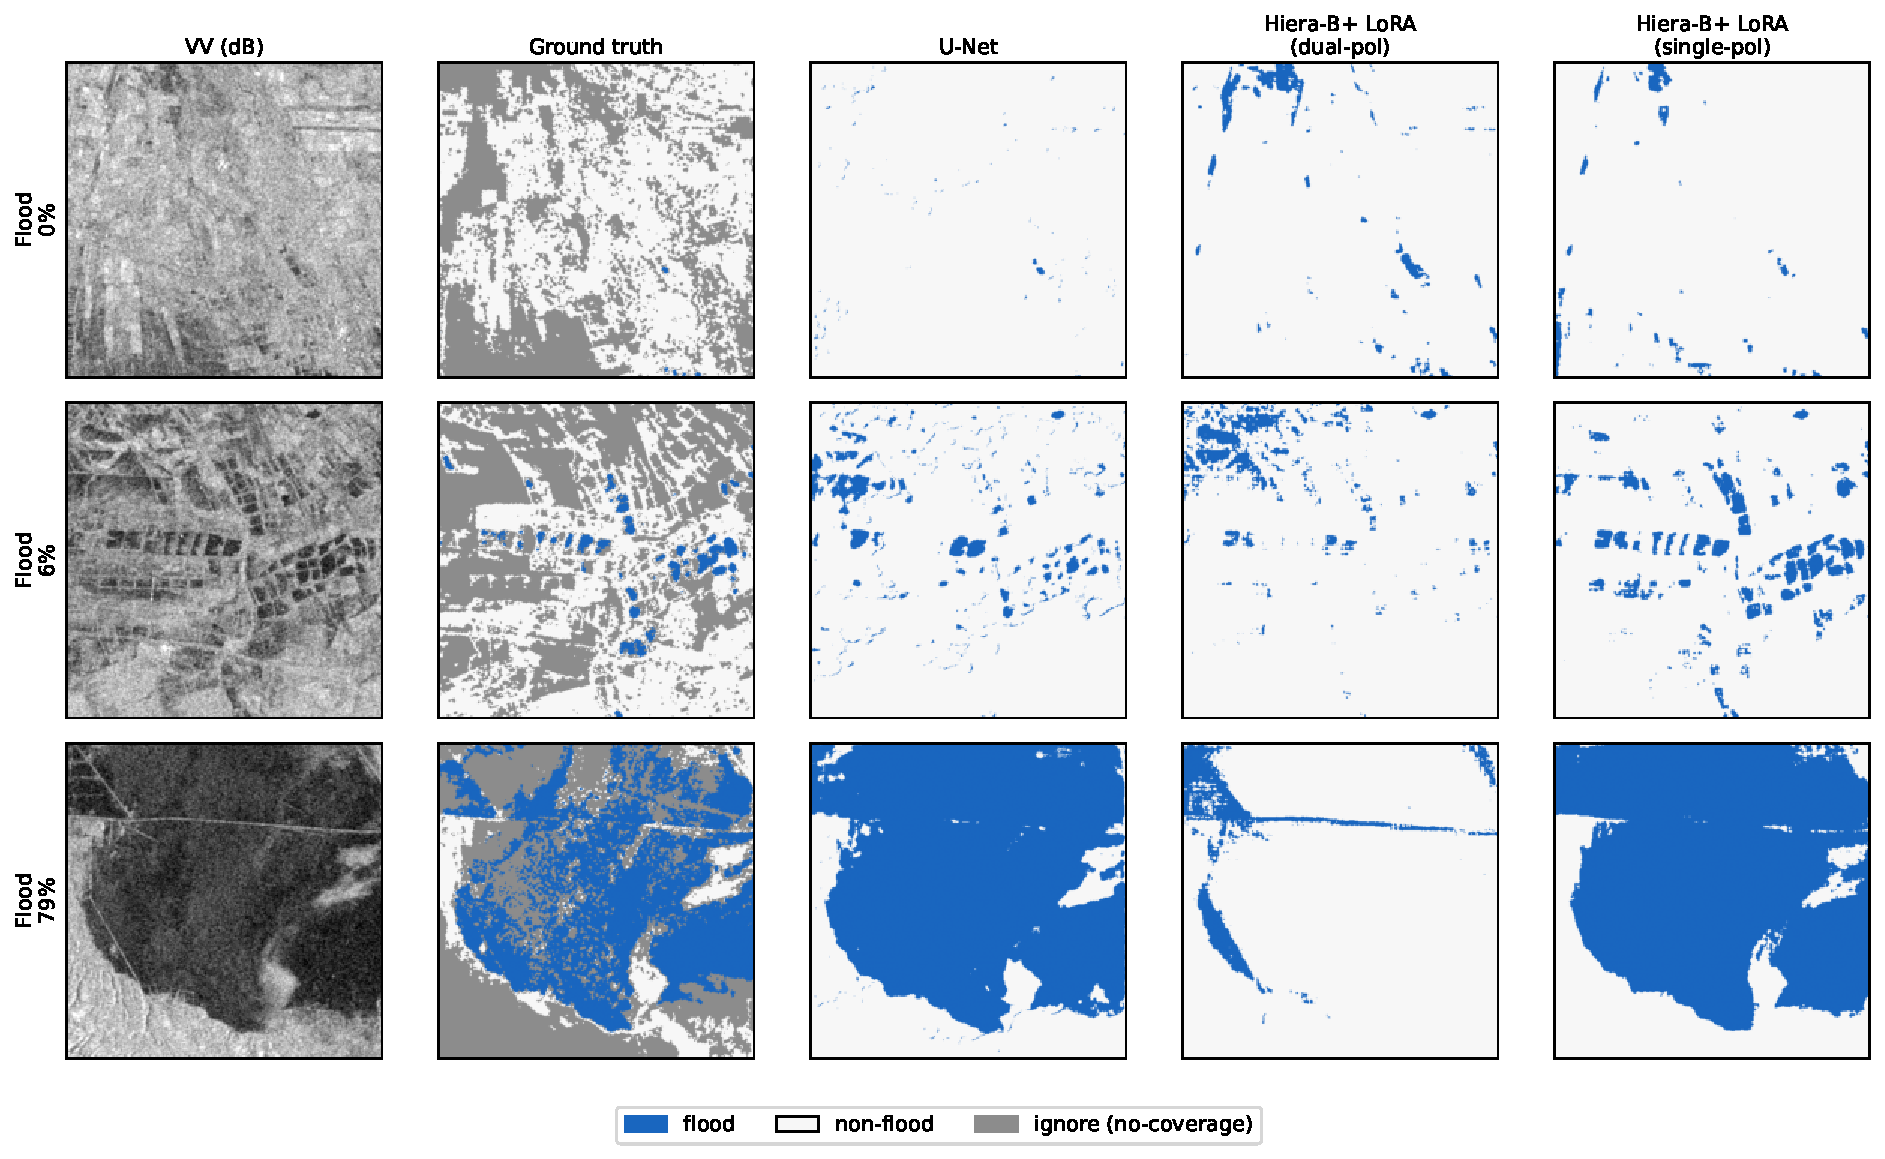
\includegraphics[width=\linewidth]{../figs/pakistan2022_overlay.pdf}
\end{center}
\vspace{0.4em}
\small
Three Pakistan-2022 chips spanning $0.2\%$, $6\%$, and $79\%$ flood fraction. Columns: VV intensity, ground truth, U-Net, Hiera-B+ LoRA dual-pol, Hiera-B+ LoRA single-pol.
\end{frame}

% ---------------------------------------------------------- Slide 5: Why?
\begin{frame}{Why? The transformer amplifies cross-polarization distribution shift}
\begin{itemize}
    \item The cross-polarization channel \emph{helps} in-distribution. Its marginal statistics on Pakistan-2022 differ from Sen1Floods11.
    \item Possible drivers: different scattering geometry, different surface conditions, different acquisition mode parameters.
    \item The SAM transformer's global attention \emph{amplifies} this distribution shift.
    \item The U-Net's local receptive fields \emph{tolerate} it.
\end{itemize}
\vspace{0.6em}
\textbf{Operational recommendation:} for new regions or events, abstain from the cross-polarization channel. Use VV only.
\end{frame}

% ---------------------------------------------------------- Slide 6: Negative finding
\begin{frame}{Negative finding: MC dropout is not per-pixel useful on OOD}
\textbf{Aggregate calibration is fine:}
\begin{itemize}
    \item ECE = $0.053$ on in-distribution test (at the well-calibrated threshold).
    \item ECE = $0.067$ on Pakistan-2022 (essentially unchanged despite the IoU collapse).
\end{itemize}
\vspace{0.6em}

\textbf{But pointwise selective-prediction curves are flat:}
\begin{itemize}
    \item Abstaining on the most uncertain pixels does \emph{not} improve IoU on the remaining ones.
    \item Aggregate calibration $\nRightarrow$ per-pixel difficulty ranking on OOD events.
    \item Contradicts the implicit assumption in prior SAR-flood uncertainty work.
\end{itemize}
\end{frame}

% ---------------------------------------------------------- Slide 7: Closing the loop
\begin{frame}{Three gaps, three closures}
\begin{enumerate}
    \item[\textbf{1.}] \textbf{PEFT comparison:} controlled head-to-head; accuracy-versus-generalization trade-off documented. AdaptFormer maximizes in-distribution IoU; LoRA family is more generalization-robust.
    \vspace{0.6em}
    \item[\textbf{2.}] \textbf{Calibration vs operational utility:} substantive negative finding. Aggregate ECE does not imply per-pixel uncertainty utility on OOD.
    \vspace{0.6em}
    \item[\textbf{3.}] \textbf{Public OOD test set:} Pakistan-2022 (39 chips, native 10\,m) released with acquisition pipeline.
\end{enumerate}
\vspace{0.6em}
\textbf{Bonus diagnostic finding:} cross-polarization is the operative OOD failure mode for SAM-family adapters.
\end{frame}

% ---------------------------------------------------------- Slide 8: Future + close
\begin{frame}{Limitations and future work}
\textbf{Honest limitations:}
\begin{itemize}
    \item Pakistan-2022 evaluation rests on 39 chips and TU Wien labels derived from a Sentinel-1 model.
    \item Stretch backbones evaluated only under Conv-LoRA.
    \item Bangladesh-Sylhet construction pipeline is released, chips are not yet built or evaluated.
\end{itemize}

\textbf{Future work:}
\begin{itemize}
    \item Empirical evaluation on the Bangladesh-Sylhet test set.
    \item Characterize the cross-polarization shift directly (incidence angle, acquisition mode).
    \item Sharper uncertainty estimators: deep ensembles, learned reject heads.
\end{itemize}
\vspace{0.6em}
\begin{center}
\Large \textbf{Thank you.}\\
\small \emph{Questions?}
\end{center}
\end{frame}

\end{document}
